% SANER 2027 RENE submission (RENE: NegativeResult)
% Compile with pdfLaTeX (Overleaf) or tectonic; see paper/overleaf_bundle/BUILD_README.md.
% fig1: SVG source under docs/research/figures_saner/; the bundle uses the vector PDF re-render (paper/_to_bundle_tex.py).
% Double-anonymous: the author block is intentionally anonymous for submission.
\documentclass[10pt,conference]{IEEEtran}
\usepackage{graphicx}
\usepackage{hyperref}
\usepackage{url}
\usepackage{amsmath}
\usepackage{seqsplit}
\usepackage{array}
\hyphenation{op-tical net-works semi-conduc-tor}
\setlength{\emergencystretch}{3em}
\begin{document}
\title{Visibility Is Not Detection: Auditing Observation Boundaries in Staged Document-Intelligence Evaluation}
\hypersetup{pdfauthor={},pdfsubject={},pdftitle={Visibility Is Not Detection: Auditing Observation Boundaries in Staged Document-Intelligence Evaluation}}
\author{Anonymous Submission}
\maketitle
\begin{abstract}
Staged document-intelligence pipelines are commonly evaluated by final answers, which conflate three distinct questions: whether an intermediate checkpoint observes a defect, whether the evaluation protocol detects it, and whether the defect is harmful under a stated equivalence contract. Long-horizon and tool-using systems motivate the same questions, but the evidence here comes from one staged document-intelligence evaluator that we audit with controlled perturbations. On a frozen public tabular corpus (95 tables, 118 controlled header perturbations in six families), 96 injections are checkpoint-visible, while the OCR-like family is unobserved on the frozen scored surface (0/13 injections across 11 clusters at every tested threshold); the existing single judge classified all 13 as referentially equivalent under its table-context contract, so benign absorption remains an alternative interpretation rather than independent ground truth. In the single-responsive-leaf construction, the unrounded flat and layered contrastive scores are a positive affine/rank transform of one another and retain identical ranks, so corresponding decisions are structurally equivalent; the zero-by-construction clean panel leaves the registered deployment operating point unresolved, which does not negate that equivalence. A preregistered stage-aligned instrumentation study (mapping, retrieval and numeric perturbations; 72 clusters, 216 injections) yields perfectly separable stage signatures (leave-one-cluster-out macro-F1 and top-1 accuracy 1.0; permutation p = 1e-4). The same direct three-leaf codebook also reaches 1.0, while the non-direct leaves reach the three-class chance level (0.3333) and, under the frozen tie-as-incorrect rule, still separate mapping from the retrieval and numeric stages without separating retrieval from numeric: the signatures reflect explicit stage-aligned instrumentation in a contract-derived construction, not emergent localization from hierarchy. A second dataflow (FinQA program perturbations; 89 rows, 30 clusters) could not be transferred: the detection predicate is defined and the counts are reproducible, but the result fields it reads are not recomputed from the perturbed program, so V=89/89, D=0/89, O=0/89 describes this carrier construction: a measurement-object mismatch that does not evidence protocol blindness. The contribution is a measurement-validity audit: visibility, detection and harmfulness are distinct constructs; the observation surface itself requires auditing per dataflow; and hierarchical organization alone does not guarantee diagnosability. The product of the audit is a boundary map and the removal of three tempting over-readings: that a visible score gap implies a performance gap, that an unobserved family is a harmful blind spot, and that separability follows from hierarchical organization; the audit is not a detector ranking.
\end{abstract}
\section{Introduction}
Document-intelligence systems are increasingly implemented as staged pipelines: a document is decoded, segmented into tables, mapped to a canonical schema, reconciled arithmetically, and queried. Such systems are typically scored by final-answer correctness. Final correctness, however, cannot distinguish a defect that was observed at an intermediate checkpoint from one that was silently absorbed by the pipeline, and it cannot reveal a defect that the evaluation protocol is itself unable to observe. Aggregating a pipeline into a single score therefore hides the property we care about first: whether the evaluation can observe the failures it is supposed to assess.
We make that property explicit with three constructs, kept separate throughout. \emph{Visibility} asks whether any instrument on the observation surface registers a defect. \emph{Detection} asks whether the protocol's decision predicate consumes that observation under its stated threshold rule. \emph{Harmfulness} asks whether the defect changes the outcome under a stated equivalence contract. These are different measurement objects: visibility is a property of instruments, detection a property of decision rules, and harmfulness a property of contracts. Confounding them produces comparisons that look quantitative but are not identified, for example, comparing protocols under different predicates and reading a sensitivity ordering into the counts. Figure 1 shows the resulting chain from injected defect to outcome harm.
\begin{figure}[t]
\centering
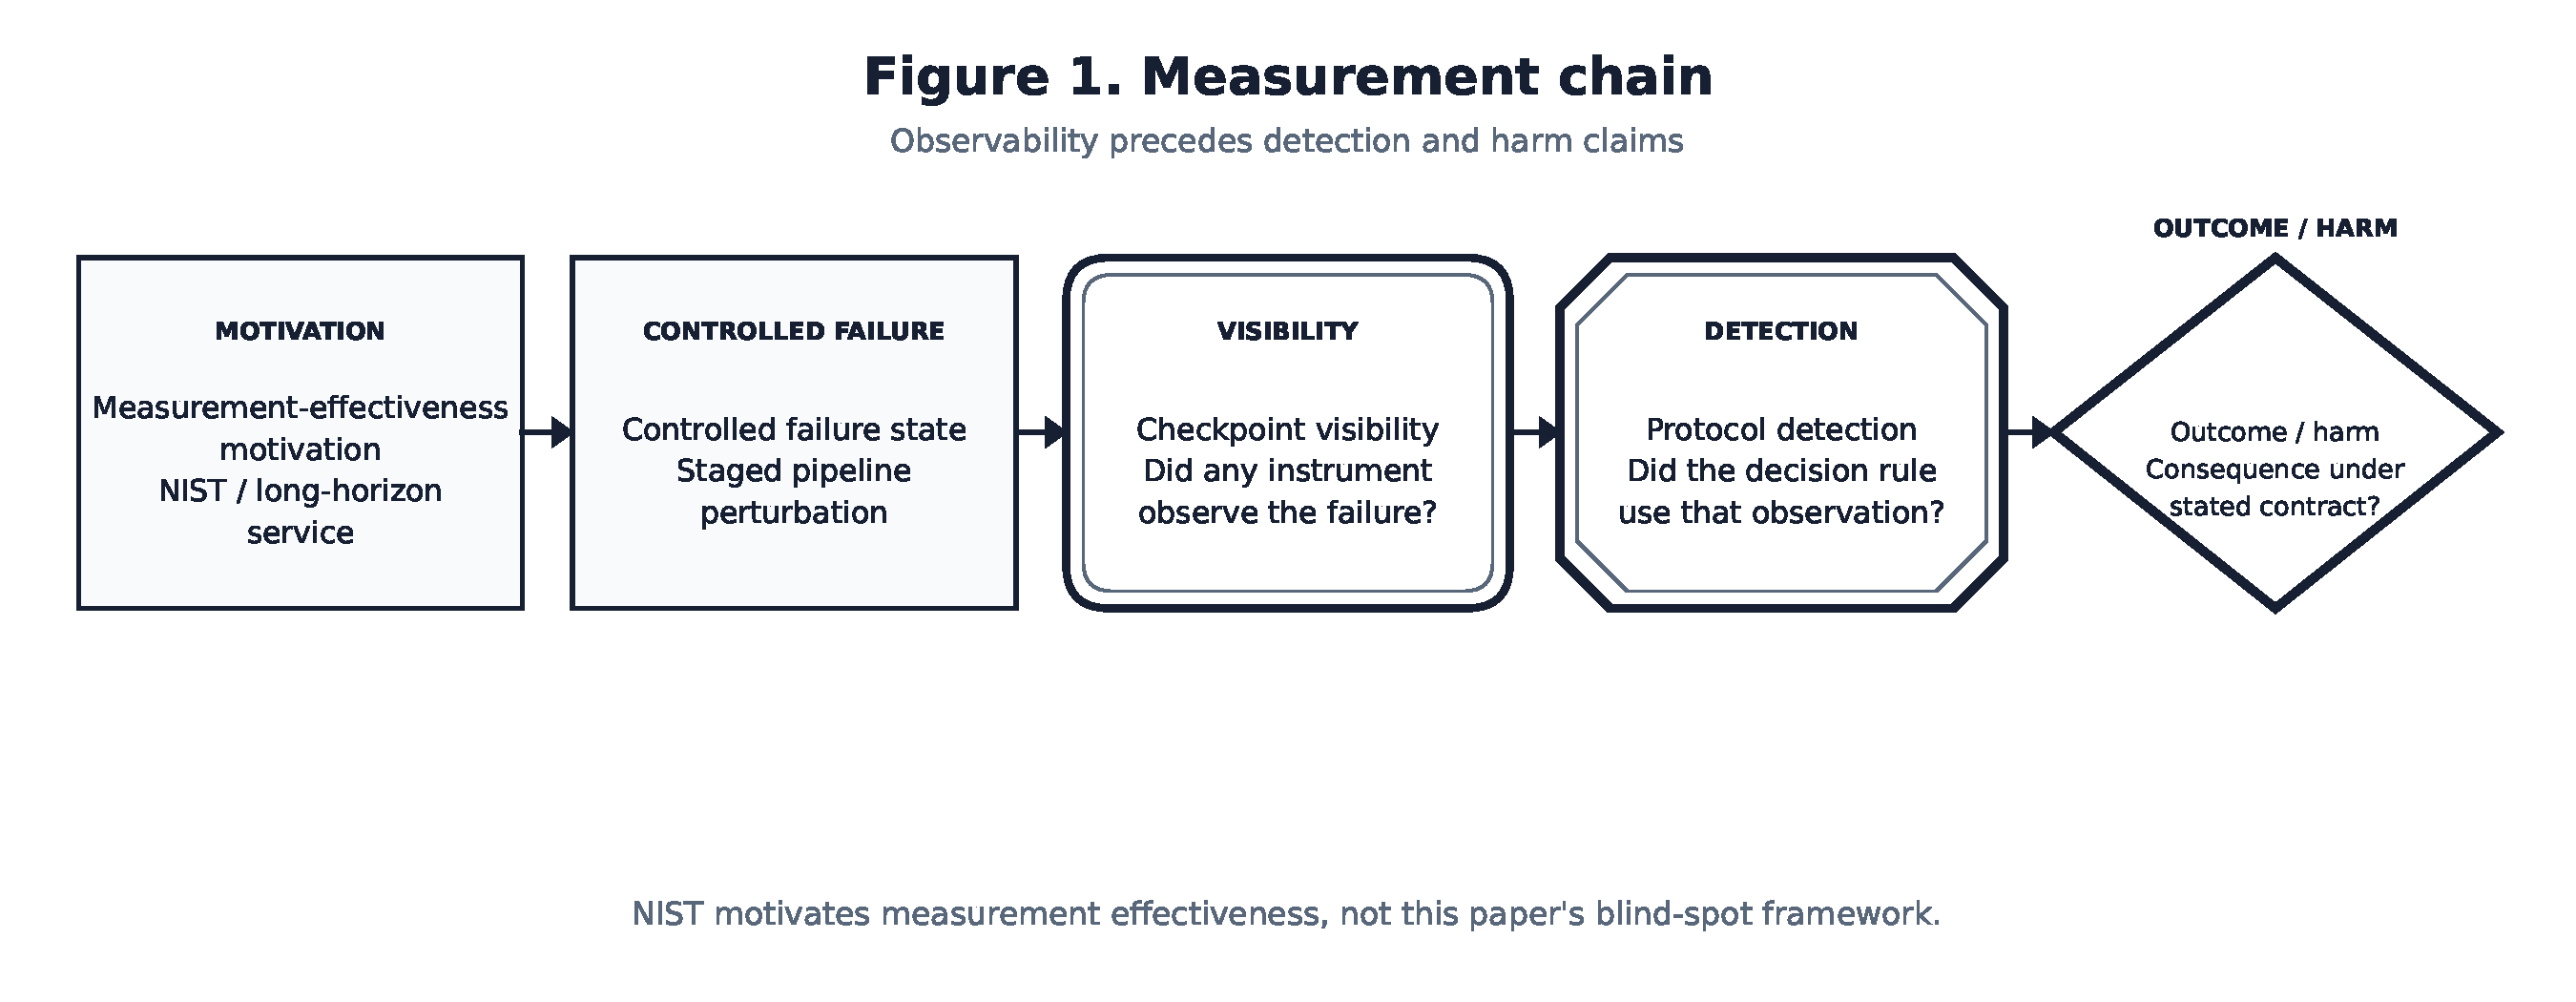
\includegraphics[width=\columnwidth]{fig1_measurement_chain.pdf}
\caption{The measurement chain. An injected failure in a staged pipeline moves through checkpoint visibility (did any instrument observe it?), protocol detection (did the decision rule consume the observation under its threshold rule?), and outcome harm (does the outcome change under the stated equivalence contract?). NIST motivates measurement effectiveness, not this paper's blind-spot framework.}
\label{fig:1}
\end{figure}
We study these distinctions through controlled fault injection on a frozen public tabular corpus, and we carry the instrument to two further settings: a preregistered stage-aligned instrumentation study on the same corpus, and a second dataflow of program perturbations (FinQA) executed under a frozen binding contract. The same pattern appears across tool-using agents and long-horizon workflows, where a final output is produced by a sequence of observable intermediate steps. The paper answers three questions per setting: (RQ1) what boundaries does the observation surface have, and how do they vary by defect family; (RQ2) are protocol comparisons on that surface empirically identified; and (RQ3) what follows when stage-aligned instrumentation is added, and what happens when another dataflow's measurement objects do not causally align with its detection predicate. Our contributions are a construct separation with quantified family-level observation boundaries; a protocol-identifiability audit that keeps a positive affine/rank structural equivalence separate from the calibration degeneracy that leaves the registered deployment operating point unresolved, together with a construction-bounded instrumentation result and its ablation; and a failed-transfer autopsy that is consistent with a measurement-object mismatch. Three of these findings are negative or boundary results: hierarchical organization adds nothing over the direct three-leaf codebook in this construction; the registered matched-FPR operating point could not be resolved on the frozen clean panel; and one defect family was never observed on the frozen scored surface. These are negative results about an instrument rather than a performance report about one pipeline: the observation surface cannot separate its own protocols at a resolved operating point on the frozen clean panel, and cannot observe an entire defect family on the frozen scored surface. We claim no universal blind spots, no hierarchy-localization, and no causal-aware checkpoint-selection method; the evidence comes from one frozen corpus with synthetic perturbations and one failed second dataflow, and no natural-failure distribution is measured. Measurement-validity and construct-validity concerns motivate auditing an evaluation surface before trusting its scores \cite{nist2023airmf}; that framing is motivation only, and NIST does not certify the metrics used here.
\section{Related Work}
\subsection{Measurement validity and construct validity}
Meta-evaluation asks whether a metric measures what it claims. Machine-translation challenge sets such as ACES test whether a metric separates genuine errors from acceptable variants \cite{amrhein2022aces,amrhein2023aces,moghe2024mtmeta}, and contextual metric meta-evaluation extends this to local, context-dependent correctness \cite{deviyani2025contextual}. Rankings can change with protocol axes, prompt subsets, seeds, or the property a metric targets \cite{kendiukhov2026ranking,du2026stability,ross2024metric}. Reliability work on LLM-as-a-judge documents position, verbosity, self-preference, and perturbation sensitivity \cite{zheng2023judging,liq2025scoringbias,lis2025llmjduge}. Construct-validity guidance frames the same concern normatively: NIST AI 100-1 asks that TEVV metrics and processes be appropriate and effective and that measurement types be reviewed for unique and meaningful information, and NIST AI 600-1 asks that construct validity be demonstrated for each metric \cite{nist2023airmf,nist2024genai}. We share the meta-evaluation aim but ask a prior question: whether the evaluation surface can observe a controlled defect at all. We keep visibility, detection, and harmfulness as separate constructs so that a protocol comparison is not read into counts that different decision rules produce.
\subsection{Testing, oracles, and diagnosability}
Mutation testing and metamorphic testing introduce controlled changes to measure whether a test or metric notices them \cite{cho2025metamorphic}; AgentChaos applies programmatic fault injection to agent systems \cite{tan2026agentchaos}. Fault-based reasoning separates whether a fault is reached, whether it changes intermediate state, and whether its effect propagates to an observable output; non-detection can arise at any of these stages, and an oracle that does not respond to a propagated effect is insensitive by construction. Process-level work evaluates intermediate behavior rather than only final success \cite{fan2026agentprocessbench,chung2026process}, and GTA-2 aggregates checkpoints recursively \cite{wang2026gta2}. We follow the mutation and fault-injection tradition but decompose non-detection into distinct mechanisms, and we treat a checkpoint forest as an evidence instrument whose diagnosability must be audited rather than assumed.
\subsection{Verified SANER RENE precedent}
The RENE track publishes reproducibility studies and negative results. Four recent papers define the surrounding practice; we describe each based on its abstract. The Limits of the Identifiable \cite{gerhold2024limits} extends deep-learning Python version identification to larger, realistic files and finds that accuracy falls from short snippets to longer segments, with import-statement analysis reaching only 30 percent, exposing limits of the approach. Does the Tool Matter? \cite{hoess2025does} compares two mining tools across ten projects and finds that even simple metrics such as commit and developer counts can differ by up to 500 percent, often from minor technical details, and hypothesizes similar uncertainty in other analysis tools. Can We Classify Flaky Tests Using Only Test Code? \cite{berndt2026flaky} evaluates three LLMs with three prompting techniques on two benchmarks and reports that classifiers are only marginally better than random, and that the test code alone does not necessarily carry enough information for a flakiness decision. Static Analysis Traces can Help Dynamic Symbolic Execution: a Replication Study \cite{kummita2026static} replicates a prior study, extends it with PhASAR-based tools and a second benchmark, and reports a conclusion different from the original: traces let KLEE find vulnerabilities about 1.4 times faster, though KLEE also confirms fewer vulnerabilities on one benchmark. These papers share our concern with measurement validity and information sufficiency; we differ in scope, auditing the observation surface of a staged document-intelligence evaluator with controlled, family-resolved injections and an explicit boundary between visibility, detection, and harmfulness.
\section{Method}
The conceptual core is a three-way audit of visibility, detection, and harmfulness; the hierarchical checkpoint forest is the evidence instrument that makes the audit reproducible.
\subsection{Evidence instrument: checkpoint forest}
We model the pipeline as two checkpoint trees. The parsing tree covers document ingestion, table structure, field mapping, and arithmetic reconciliation. The QA tree covers retrieval grounding, faithfulness, numeric correctness, citation quality, and appropriate refusal. Together the trees contain 12 scored leaves.
The twelve scored nodes are five in the parsing tree (document status, document throughput, table regression, field hit-rate, reconciliation equations) and seven in the QA tree (retrieval contract, faithfulness judge, numeric contract, number grounding, citation judge, refusal judge, refusal contract), per the frozen checkpoint-tree configuration v0.1.0 (listed in the artifact manifest). The visibility audit exercises the parsing-tree leaves whose evidence is the mapping and regression artifacts; under the frozen drop rule (drop = (H\_orig - H\_inj) x 10, threshold 2.0) only the field hit-rate leaf responds to header drift, while QA-tree leaves keep their frozen evidence and the QA arm is reported separately (12 calls to the same judge). Additional localization value therefore remains unestablished in the current instantiation. In Table 1, the label \emph{Pruned parsing-root drop} denotes exactly this operation: the parsing root is collapsed to its single input-responsive leaf (the field hit-rate leaf) and the drop rule above is applied there.
Each leaf receives a score in [0,10]. Contractible properties use deterministic checks; semantic properties use a 0–5 judge score mapped to [0,10]. Sibling weights are normalized locally before bottom-up aggregation. Missing evidence is explicit: the parsing tree assigns 0, whereas the QA tree assigns a neutral 5. Hinge leaves affect the stability verdict, not the missing-evidence score. Every leaf stores its evidence and degradation reason.
For node n with children C(n), the recursive score is
\[
S(n)=\sum_{c\in C(n)} \frac{w(c)}{\sum_{j\in C(n)}w(j)}S(c).
\]
For a leaf, S(n) is the mapped contract or judge score. A tree is stable only when at least 90\% of its leaves exceed the selected threshold and every hinge leaf scores at least 7. The implementation is deterministic once the evidence artifacts are fixed.
\subsection{Separating visibility, detection, and harmfulness}
Visibility is defined relative to the selected checkpoint evidence surface, whereas protocol detection may use a different downstream signal.
The primary conceptual structure is the following visibility-by-detection matrix:
\begin{table}[t]
\centering
\small
\setlength{\tabcolsep}{3pt}
\begin{tabular}{>{\raggedright\arraybackslash}p{0.293\columnwidth}>{\raggedright\arraybackslash}p{0.293\columnwidth}>{\raggedright\arraybackslash}p{0.293\columnwidth}}
\hline
Checkpoint evidence & Protocol detects & Protocol does not detect \\
\hline
Visible & Detected visible defect & Visible but undetected \\
Not visible & Detection through a different signal or predicate & Silently absorbed or unobservable \\
\hline
\end{tabular}
\end{table}
Harmfulness is orthogonal to this matrix and is annotated separately as harmful, equivalent, or unresolved under the selected equivalence criterion.
For an injected defect d, visibility and protocol detection are separate observations:
\begin{itemize}
\item \textbf{Detected:} the selected protocol satisfies its detection predicate, which may test a mapping change or a score threshold.
\item \textbf{Visible but not detected:} the checkpoint exposes a difference, but the selected protocol does not satisfy its detection predicate.
\item \textbf{Silently absorbed:} normalization or matching preserves the canonical correspondence, so that the checkpoint does not expose the perturbation.
\end{itemize}
Harmfulness is a separate, \textbf{equivalence-dependent} judgment, not a mutually exclusive visibility outcome: canonical-form preservation and reader-referent recoverability need not agree.
The defect visibility profile reports visibility separately for each family. This preserves information lost by a single mutation score and distinguishes a missing checkpoint from a genuinely robust stage.
\subsection{Evaluating the evaluator}
We compare four protocols on frozen evidence: end-to-end roots, a flat leaf average, hierarchical expert weights, and hierarchical searched weights. We measure table-level detection, injection-level detection, mean separation between clean and perturbed states, worst-family behavior, localization, and evaluation cost. Because raw thresholds can manufacture differences, we separately audit (i) structural score/ranking equivalence and (ii) whether a matched-FPR operating point is identifiable from clean scores alone.
The audit further varies the injection seed, visibility threshold, matching algorithm, and scoring normalization. A semantic-judge arm is evaluated separately and never substituted for deterministic evidence when a contract exists.
\subsection{Stage-aligned instrumentation and the second dataflow}
The evaluation-track instrument is a two-root checkpoint forest whose twelve leaves map deterministic or judge-derived evidence to a 0–10 score (Section 3.1). To test whether stage-aligned instrumentation carries stage information, we preregister a separate controlled study on the same corpus. Each stage contract perturbs one operation: a header token is replaced (mapping stage M), required source blocks are removed from the retrieval bundle (retrieval stage R), or one numeric operand is broken while labels, schema and identity are preserved (numeric stage N). Every cluster contributes three deterministic injections, and each injection is scored on the same twelve-leaf surface, producing a binary response vector; 24 clusters per stage give 72 clusters and 216 injections. The study is frozen before results (hash receipt) and evaluated leave-one-cluster-out. The same document defines the protocol's deliberate boundary: response predicates are written from the stage contracts, so the construction is explicitly instrumented and its separability must be interpreted within that construction.
The second dataflow is a program-perturbation corpus built from FinQA reasoning steps. Perturbations act on a step's operator or argument fields while the downstream result fields are not recomputed; the observation objects are visibility (does the injected change appear in the observed source fields), detection (does the frozen detection predicate move), and outcome (does any downstream outcome field change). The execution contract binds artifact hashes before scoring, and no threshold or convention search is permitted. Section 4.5 states the execution boundary; Section 5.6 reports what happened and what it does and does not establish.
\section{Experimental Setup}
\subsection{Corpus and perturbations}
The study uses a frozen public tabular base and contains no client data. It includes 95 tables and 118 synthetic injections across six header-drift families. Schema and header matching are the perturbation carrier here; the object of study is the evaluation protocol's observation boundary. Each injected record preserves its source table, family, seed, changed field, and expected observation surface.
Concretely, the base is the frozen drift-v0 table set derived from public TAT-QA tables (listed in the artifact manifest by content hash); the corpus was frozen before this study's data gates and no new TAT-QA use is introduced. The perturbations are the fully synthetic injection map (listed in the artifact manifest by content hash; deterministic, seed 42, ratio 0.3). The matcher used in the audited pipeline is the greedy header matcher (listed in the artifact manifest); the cross-matcher audit adds greedy-normalized, Hungarian, and Hungarian-normalized configurations. Semantic leaves are scored by the judge pipeline (listed in the artifact manifest), i.e. Qwen3.6-35B-A3B (Q4\_K\_M GGUF) served locally, with 0–5 dimension scores mapped to [0,10]. The primary threshold grid is
\[
\Gamma=\{0.2,0.3,0.5,0.7,0.9\}.
\]
The OCR-like family contains 13 single-token, lowercase Levenshtein-distance-one substitutions with unchanged column values. These properties are mechanically recomputed before interpretation.
\subsection{Baselines and controls}
The protocol baselines are end-to-end scoring, flat leaf scoring, and hierarchical scoring with expert weights. Weight-search controls include equal weights, expert weights, 30 random trials, greedy coordinate ascent, particle-swarm optimization (PSO), and a minimax objective. Assignment controls compare greedy matching with Hungarian global assignment and include a positive solver test.
\subsection{Statistical discipline}
We freeze inputs and decision criteria before reading each result. Confidence intervals are reported on table-level clustered units where available (percentile bootstrap over the 95 table units, seed 20260830; endpoints on the k/95 grid for the 95-table arm). Seed sensitivity uses three injection seeds. For the clean-only matched-FPR audit, threshold selection may use clean scores only; injected and harmful outcomes are prohibited from calibration. Because the frozen clean supports are degenerate, the registered deployment operating point is left unresolved rather than forced into an empirical equality. The 2,382 clean records are the usable (table\_uid, column) rows of the non-injected source tables in the frozen clean-input set, with fold assignment = sorted(table UID) index modulo 5. Null and adverse findings are retained rather than relabeled as improvements.
\subsection{Multi-leaf stage-aligned protocol}
The stage-aligned study uses the same frozen tabular base and the same twelve-leaf surface. Stage contracts and injection generators are deterministic; clusters are selected by an outcome-blind hash rule (seed frozen before results), and the pre-result freeze receipt binds the corpus, the generator, the runner and the environment by hash. Response predicates are contract-derived: for M the directly targeted parse leaves move; for R the retrieval leaf moves; for N the reconciliation leaf moves. Baselines are the metric-specific chance top-1 (1/3) and majority macro-F1 (1/6); uncertainty uses leave-one-cluster-out evaluation with 10,000 cluster-bootstrap resamples and a 10,000-replicate permutation null, both seeds frozen. The ablation re-scores the same rows with (i) the full twelve-leaf vector, (ii) the fixed three-direct-leaf codebook, (iii) non-direct leaves only, and (iv) a single any-response scalar.
\subsection{Second-dataflow execution boundary}
The FinQA second flow executes a frozen step-perturbation corpus under a hash-bound binding contract: 89 rows over 30 clusters, with per-row runtime bindings and a full trace map verified before scoring. The perturbation writes operator/argument fields; the observation vector records visibility, detection and outcome per row. Because downstream result fields are not recomputed from the mutated program semantics by construction, a zero detection count in this execution is not an estimate of detection ability; Section 5.6 states the resulting measurement-object boundary and the alternatives the evidence does not exclude. No threshold search, convention selection, or source-operator substitution is permitted in this flow.
\section{Results}
\subsection{Visibility depends on defect family}
Checkpoint-level analysis makes 96/118 injections visible, but the aggregate hides a large family effect. 0/13 OCR-like injections were visible across 11 table clusters under all five thresholds; all 13 were invisible under this observation criterion. Other families range from 0.81 to 1.00 visibility at the primary setting. For uncertainty, the injection-level reference estimand is 0/13 with an exact binomial 95\% interval of [0, 24.71\%] under an independent-injection assumption; the distinct table-level event estimand is 0/11 with an exact binomial interval of [0, 28.49\%]. The latter is not a clustered confidence interval for injection-level visibility. Figure 2 reports the full family-by-threshold visibility profile.
\begin{figure}[t]
\centering
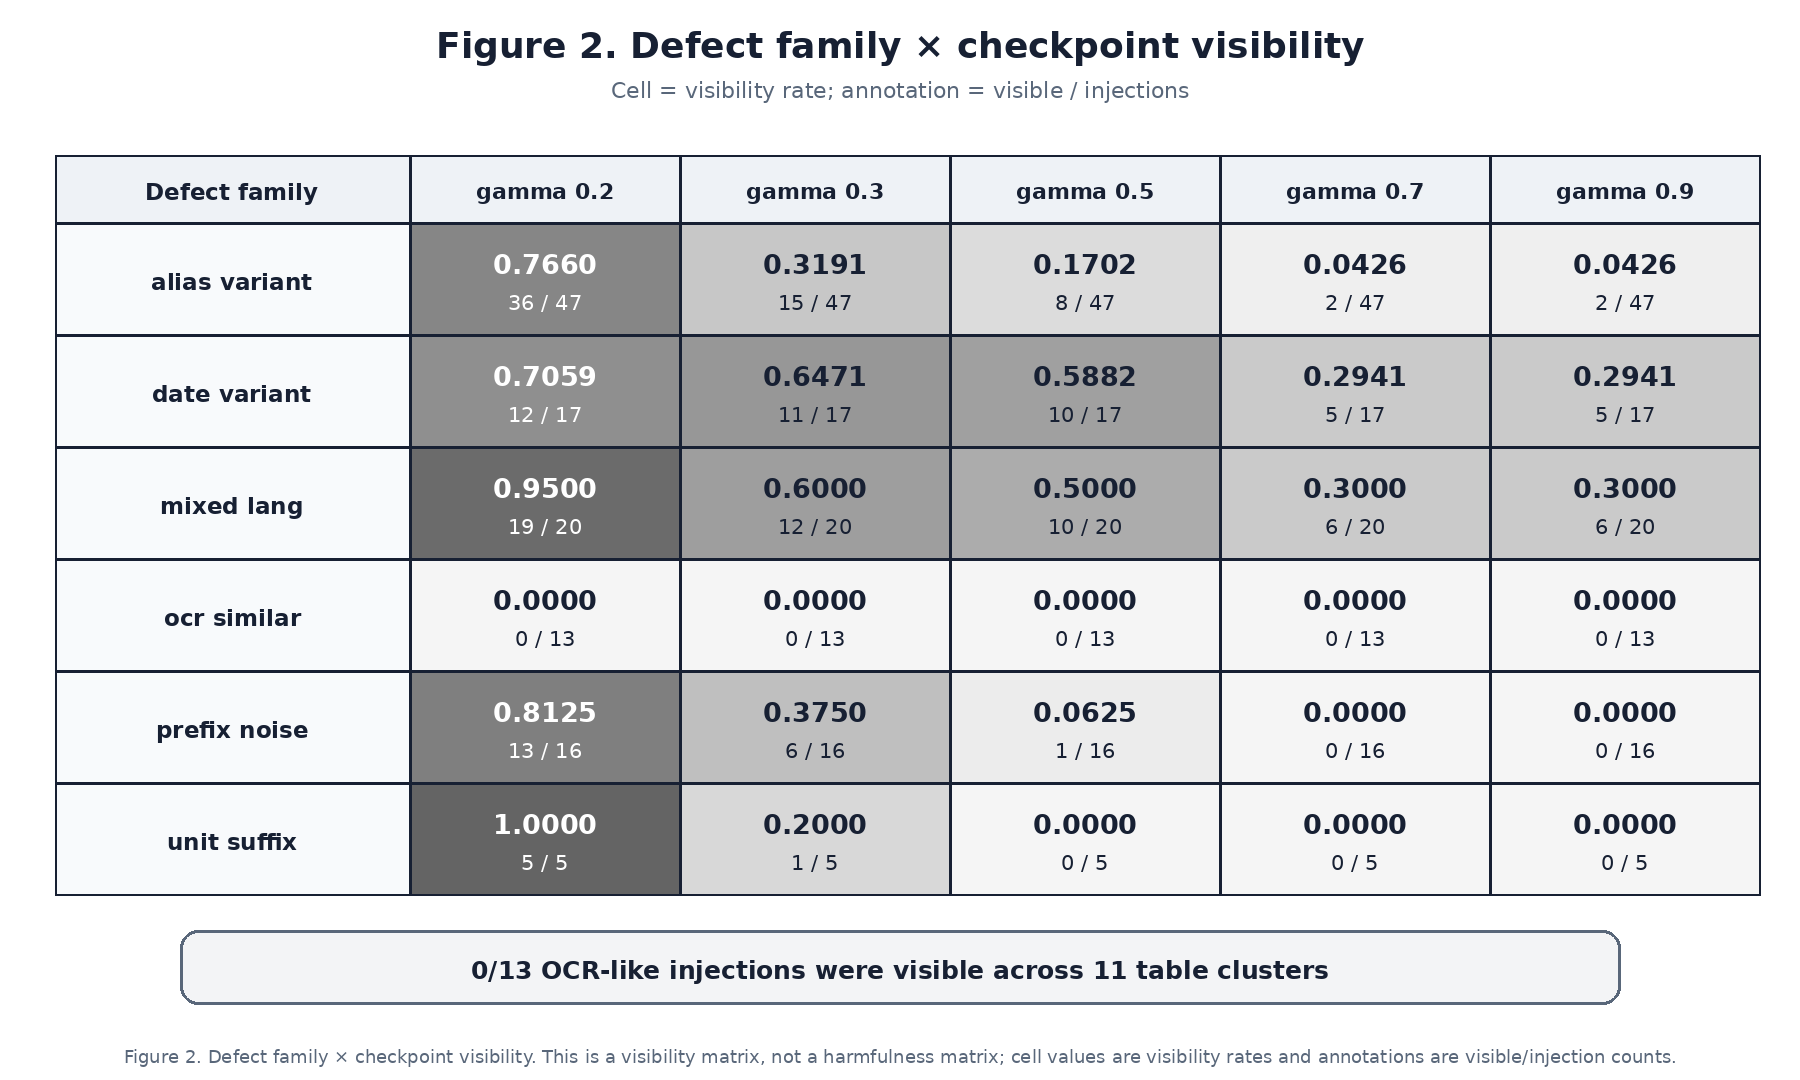
\includegraphics[width=\columnwidth]{fig2_family_visibility_matrix.png}
\caption{Defect family × checkpoint visibility. Cell values are visibility rates at each threshold, annotated with visible/injection counts; the OCR-like family is 0/13 across 11 clusters at every tested threshold. This is a visibility matrix, not a harmfulness matrix.}
\label{fig:2}
\end{figure}
The family unobserved on the frozen scored surface remains the same under four edit-distance matcher configurations. However, the ordering of visible families is not invariant: changing the score normalization causes five class flips, all within the date-variation family, whereas switching from greedy to global assignment causes no flips. Thus, the existence of a family unobserved on the frozen scored surface is stable within the tested matcher family, but the full ranking is protocol-dependent.
The harmfulness label is also criterion-dependent, and our record contains two comparison kinds that should not be pooled. In the first kind, seven paired judge-versus-standard comparisons yield four disagreements; the two standards differ in the criterion they apply, with the standard asking whether the canonical form and canonical truth survive and the judge asking whether a reader can recover the same referent. In the second kind, a single visibility-versus-equivalence comparison contrasts deterministic channel evidence with standard equivalence, and that case carries no judge call. Because the two kinds measure different objects, we keep the raw cases and report neither a pooled disagreement rate nor a mechanism that would exclude case-level noise. In particular, the existing single judge, applying its table-context reader-referent contract, classified all 13 OCR-like perturbations as referentially equivalent. That supports benign absorption as an alternative interpretation of the non-response; it is not independent ground truth, and non-response alone does not establish harmful false negatives. We therefore report that this family is unobserved on the frozen scored surface, while treating whether that absence is harmful as a boundary question.
\subsection{The raw hierarchy gap is a threshold-placement artifact}
The raw detection counts are not evidence of protocol discriminability. Table 1 compares three transferable protocols under different decision predicates: end-to-end detection tests whether the final mapping text changes, whereas flat and hierarchical scoring use frozen score-drop thresholds. A changed source-header string can therefore count as end-to-end detection even when the canonical match is preserved, explaining why 112/118 exceeds the 96/118 visibility count. Table-level counts apply all assigned injections together, whereas injection-level counts apply one perturbation at a time; the 20 detected tables and 13 individually detected injections are not nested counts. At the frozen threshold, hierarchical scoring is not a more sensitive detector.
\textbf{Table 1. Protocol-level detection under different decision predicates.}
\begin{table}[t]
\centering
\small
\setlength{\tabcolsep}{3pt}
\begin{tabular}{>{\raggedright\arraybackslash}p{0.220\columnwidth}>{\raggedright\arraybackslash}p{0.220\columnwidth}>{\raggedright\arraybackslash}p{0.220\columnwidth}>{\raggedright\arraybackslash}p{0.220\columnwidth}}
\hline
Protocol & Detection signal & Tables detected & Injections detected \\
\hline
End-to-end & Final mapping change & 95/95 (1.0000) & 112/118 (0.9492) \\
Flat & Field-hit-rate drop & 75/95 (0.7895; 95\% CI [0.6947, 0.8737]) & 85/118 (0.7203) \\
Hierarchical, expert weights & Pruned parsing-root drop & 20/95 (0.2105; 95\% CI [0.1263, 0.2947]) & 13/118 (0.1102) \\
\hline
\end{tabular}
\end{table}
The raw flat-hierarchical gap does not establish inferior ranking quality. In the current single-responsive-leaf construction, the unrounded hierarchical contrastive score is a positive rescaling of the flat contrastive score, with fitted slope approximately 0.375, and the recorded scores retain identical ranks; corresponding decisions, and by implication their ROC geometry, therefore coincide, and corresponding thresholds satisfy theta\_H = 0.375 theta\_F. This is a structural equivalence of the two protocols' decisions, not a newly calibrated performance estimate; the diagnosis is deliberately narrow: it explains why the raw protocol gap cannot be read as a ranking difference, and it is not offered as a general algebraic result about hierarchical evaluation. Separately, the registered deployment operating point remains unresolved: the derived clean-only reanalysis contains 2,382 usable clean records whose score supports are exactly \{0\}, so every positive threshold has an observed FPR of zero and the clean panel cannot select a unique operating point. That calibration degeneracy does not negate the structural equivalence, and it is a statement about the current clean-only procedure, not a general claim that matched-FPR comparisons cannot be made; the registered strict predicate FPR = alpha and the tolerance predicate FPR <= alpha also remain distinct. Selecting a threshold by harmful TPR would violate the clean-only contract. Historical fixed-threshold sensitivity evidence is retained in Appendix A.4, but the old [0,0] interval is not a clean-calibrated confirmatory result. When more than one leaf varies with the input, neither affine nor ranking equivalence is guaranteed.
The 118 injections close at the checkpoint level as 96 visible plus 22 silently absorbed; by family (injections / visible / absorbed): alias variant 47/43/4, date variant 17/15/2, mixed language 20/20/0, OCR-like 13/0/13, prefix noise 16/13/3, unit suffix 5/5/0 (frozen artifact listed in the evidence ledger). The protocol-level counts in Table 1 are measured on different signals and are therefore not a partition of the 96.
We label the affine-equivalence observation a degenerate-case result: it fixes the interpretation of the raw gap under the current single-varying-leaf construction and does not establish affine equivalence of the protocols in general.
\subsection{Sensitivity and reproducibility}
The identity of the family unobserved on the frozen scored surface is stable across the threshold grid. The absolute between-family range shrinks at high thresholds, as expected when one changed header contributes at most 1/n for a table with n canonical headers. The literal preregistered range criterion fails at 0.7 and 0.9, and this failure is reported.
Across three injection seeds, flat table-detection rates are 75/95 = 0.7895, 76/97 = 0.7835, and 68/90 = 0.7556. Their spread is 0.0339; the denominator-weighted pooled rate is 219/282 = 0.7766 with a percentile bootstrap 95\% interval of [0.7270, 0.8227] over the pooled 282 table units (seed 20260830; endpoints on the k/282 grid). The seed-42 run reproduces the frozen artifact byte-for-byte.
Judge calibration covers 120 leaf-state cells; this calibration window is distinct from the 28-case semantic boundary analysis reported in Section 6. In the control-state comparison, rejudged summaries of historical 0–5 judgments differ from the frozen dimension means by at most 0.5, meeting the preregistered consistency expectation. This checks reproduction of aggregate dimension scores, not agreement between judges re-evaluating the same original answers. On the derived 0–10 root scale, control roots differ by at most 0.22, while individual leaves can move by as much as 7.0. Agreement is therefore an aggregate observation, not evidence of cell-level interchangeability.
\subsection{Weight search produces an informative null}
PSO and greedy coordinate ascent reach the same mean separation of 1.432574. PSO repeats the result on all five seeds but requires 7,650 evaluations, compared with 67 for greedy search. A minimax variant improves worst-case separation to 0.35714 while reducing mean separation to 1.25605. We therefore do not claim PSO superiority. The result instead shows that objective choice matters more than optimizer sophistication in the present search space.
\subsection{Stage-aligned instrumentation: separable signatures and their boundary}
\begin{figure}[t]
\centering
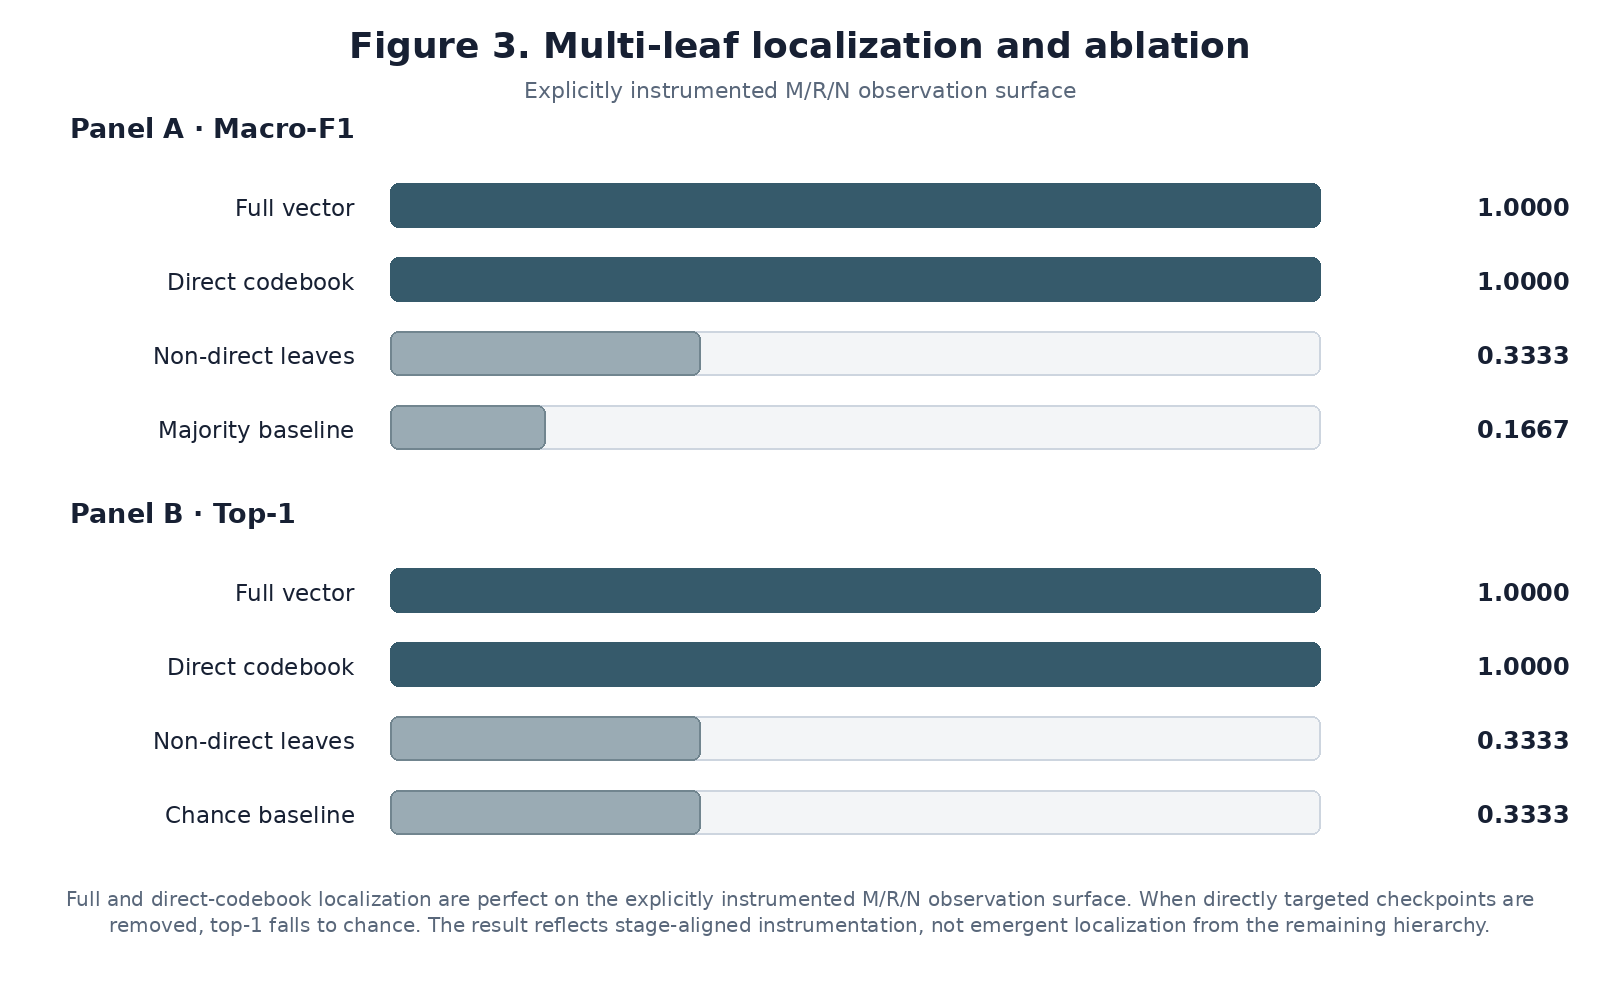
\includegraphics[width=\columnwidth]{fig3_localization_ablation.png}
\caption{Multi-leaf localization and ablation. Perfect full-vector and direct-codebook bars are construct-sensitive on the explicitly instrumented controlled M/R/N observation surface. After directly targeted checkpoints are removed, non-direct top-1 equals chance (0.3333); under the frozen tie-as-incorrect rule these leaves still separate mapping from the retrieval and numeric stages without separating retrieval from numeric. Non-direct macro-F1 equals the uniform-class macro-F1 baseline (0.3333); the majority-class macro-F1 reference (0.1667) is plotted. The result reflects stage-aligned instrumentation, not emergent localization from the remaining hierarchy.}
\label{fig:3}
\end{figure}
The preregistered stage-aligned study separated the three controlled stages perfectly on the explicitly instrumented surface: leave-one-cluster-out macro-F1 and top-1 accuracy are 1.000 with cluster-bootstrap 95\% intervals [1.0, 1.0] and permutation p = 1/10001 = 1e-4, with zero ties and zero errors, against metric-specific baselines (chance top-1 1/3; majority macro-F1 1/6). The per-stage response profiles are disjoint within the construction: M moves the field-hit and table-regression leaves, R moves the source-required leaf, and N moves the reconciliation leaf. Figure 3 reports the localization and ablation outcome.
That positive result carries its boundary in the same rows. Re-scoring the identical 216 injections with the fixed three-direct-leaf codebook also yields macro-F1 and top-1 of 1.000; the non-direct leaves alone fall to 0.3333 with a tie rate of 0.6667, which is the three-class chance level and the uniform-class macro-F1 baseline; under the frozen tie-as-incorrect rule they distinguish the mapping stage from the retrieval and numeric stages but do not distinguish retrieval from numeric, so they carry partial rather than no stage information. A single any-response scalar collapses to 0.0 with ties everywhere. Eight of the twelve leaf columns are identically zero over all injections. Perfect separability therefore reflects explicit stage-aligned instrumentation in a contract-derived construction, not emergent localization from the remaining hierarchy, and the positive result is reported together with this ablation. Per-stage estimates are descriptive at this sample size; the population is the frozen controlled injection set, not a natural-failure distribution.
\subsection{A second dataflow: a failed transfer consistent with a measurement-object mismatch}
The FinQA second flow produced V = 89/89, D = 0/89 and O = 0/89: every injected change was observable on the mutated source fields, the frozen detection predicate never moved, and no downstream outcome field changed. The detection predicate here is defined and executable, and these counts are reproducible; what the perturbation does not do is regenerate the downstream result fields that the predicate reads. The zero detection count therefore describes this carrier construction rather than an estimated detection ability, and the mismatch is one of measurement objects, not of predicate definition. The formal result class is a mixed second-flow outcome; the accepted interpretation is a measurement-object mismatch, recorded in a separate autopsy. We therefore treat causal alignment of measurement objects as a design requirement for future transfers, not as a validated law. Scorer non-portability, threshold non-transfer and corpus shift are not excluded by this evidence, and no transfer, blindness or semantic-correctness claim is made from this flow.
\subsection{Boundary case outside the main contribution}
This case is not part of the evaluation-track contribution; it only marks the boundary between evaluation-track evidence and the broader reasoning-step question.
In a compact feedback example, a gain–collateral gate rejects all 7 adversarial high-confidence mappings and all 5 expanded-collision candidates. Across 15 collision tables, the gated-minus-ungated mean paired difference is 0.05 with a 95\% interval of [0, 0.1056], while the exploratory pooled comparison is 7/40 versus 4/40 with exact McNemar p=0.375. This is not an efficacy claim.
\section{Discussion and Limitations}
\subsection{Scientific limitations}
The main finding is methodological. Aggregate evaluation can hide both system defects and defects unobserved on the scored surface. A checkpoint forest makes evidence decomposable, while a visibility profile shows which defect families are observable. Yet structure alone does not guarantee sensitivity: in the current single-responsive-leaf construction, flat and hierarchical scores are affine/rank-equivalent, so their decisions coincide, while the registered deployment operating point remains unresolved because the clean-only calibration panel is degenerate.
Four limitations bound the claim. First, the evidence comes from one public tabular corpus with synthetic perturbations; no cross-domain generalization is claimed. Second, the OCR-like family is unobserved on the frozen scored surface, but whether each perturbation is harmful depends on the equivalence definition; a single judge classified all 13 of those cases as referentially equivalent under its table-context contract, which is an alternative interpretation of the non-response rather than independent ground truth. Third, the semantic boundary analysis uses one judge on 28 cases; mixed-language and unit-suffix families receive no calls in that window (a separate window from the 120-cell judge calibration of Section 5.3). Fourth, under shared-header overlays the oracle correctness ceiling changes from 20/21 = 0.952381 to 40/67 = 0.597015 (the two figures use different denominators; this is not a ratio comparison), while global assignment changes no decision, locating the problem in score construction rather than allocation.
\subsection{Deferred independent evidence}
A preregistered second-dataflow extension did not satisfy its structural prerequisites and is therefore not used as evidence. A preregistered independent-scorer route triggered its pre-registered stop condition and is therefore not reported as a capability result. The criterion-relativity claim remains limited to the current evaluator and corpus; the detailed governance record is retained in Appendix A.
\subsection{Integrating the observation surfaces}
Three results share one structure. First, the frozen evaluation surface has a family-level boundary: the OCR-like family is unobserved across all tested thresholds and clusters while the remaining families are observed at rates from 0.81 to 1.00. Second, adding observations along the failure path changes what is diagnosable: with stage-aligned instrumentation the controlled stages separate perfectly, and when the directly targeted leaves are removed the remaining leaves still separate the mapping stage from the retrieval and numeric stages without completing the three-way split, so what a surface can diagnose is set by its instrumentation, not by its organization. Third, when another dataflow is measured with a predicate that does not share its perturbation's object, the comparison is not estimable: the FinQA predicate is defined and its counts are reproducible, yet the result fields it reads are not regenerated from the perturbed program, so the correct conclusion is a boundary, not a performance number. Together they support a measurement-validity discipline: audit an observation surface and its measurement objects per dataflow before trusting aggregate scores. The evidence remains bounded by one frozen public corpus with synthetic perturbations, one controlled instrumentation study, no natural-failure distribution, harmfulness defined relative to an equivalence contract, and a second dataflow that failed for measurement-object reasons. The paper's claims hold within these limits.
\section{Conclusion}
Final correctness cannot tell whether a defect was observed at an intermediate checkpoint, silently absorbed, or invisible to the evaluator itself. We introduced a three-way audit of visibility, detection, and harmfulness, implemented with hierarchical checkpoint evidence and per-family visibility profiles. On 118 controlled injections in this evaluator, observability and detection depend strongly on defect family and decision protocol. The central result is structural rather than a detector ranking: in the single-responsive-leaf setting the two protocols' decisions are structurally equivalent, while the registered deployment operating point remains unresolved because the clean calibration panel is degenerate. Evaluations of staged document-intelligence pipelines should therefore report the protocol's own observation boundary, validity limits, and reproducible evidence chain alongside aggregate system performance; carrying this discipline to other staged systems is a design recommendation, not a measured long-horizon result.
\section{Data Availability}
The evaluation corpus is derived from the public TAT-QA tables; the frozen drift-v0 injector, the checkpoint-tree configuration, the aggregation code, and the analysis scripts are prepared for release as an anonymized artifact, with the exact revisions and content hashes listed in the artifact manifest. The FinQA second-flow execution is described by its frozen activation record and is reproducible from the scripts prepared for release; the semantic-judge model weights are third-party and are cited rather than redistributed. Study materials and intermediate artifacts are planned to be made available to reviewers through an anonymized repository at submission time; that repository and its persistent DOI are not yet established. No client or proprietary data is used.
\bibliographystyle{IEEEtran}
\bibliography{saner_rene_references}
\appendix
\section{Deferred independent-evidence record}
This appendix preserves the internal evidence and preregistration record for deferred extensions. These materials are boundary records, not evaluation-track results.
\subsection{A.1 Reinstatement criteria}
Reinstatement criteria, not a timeline: the deferred arms return only when (i) a second dataflow with a table layer passes the source-identity and split gates with UID-disjoint layers, and (ii) a second scorer independent of the local judge reproduces the leaf-state cells; until both hold, the arms remain preregistered-but-unreported.
\subsection{A.2 Second-dataflow record}
Progress against criterion (i) is now measurable, clause by clause. Three corpora answer different clauses and are named separately: the acquisition corpus (FinQA, taken under the approved minimal scope), the action corpus (a schema-matching benchmark of ten table pairs), and the transfer corpus whose missing table layer triggered the original deferral. The source-identity gate passed on 2026-09-25 for the acquisition corpus, with per-file digests recorded. Its table layer is present and uniform: all 7134 examples carry a non-empty rectangular table whose first row is entirely string-valued, with two to eleven columns, so the clause that deferred the transfer corpus, the absence of a table layer, does not apply to the acquisition corpus. A deterministic, label-blind split instrument now assigns layers whose independence clusters are report-level rather than dataset-level, and on the acquisition corpus the four role layers are geometrically fillable, with 2409 lineage UIDs over 768 report clusters at full population. The split gate is nonetheless not passed: the acquisition corpus has its own gate and sealed partitions withheld because its registered role list does not include them, while the action corpus, which is the one that carries an action vocabulary, contains ten table-pair clusters and under the frozen hash-threshold bucketing rule leaves the development layer empty, yielding ten independent units. The remaining gap is structural rather than incremental, and it belongs to the label gate, not to criterion (i): the acquisition corpus publishes no official canonical vocabulary for table columns, so action labels could only be constructed by inventing a schema. Here, a table layer makes samples definable; it does not supply the gold those samples need.
\subsection{A.3 Independent-scorer record}
Criterion (ii) has not been tested, and one candidate route toward it was stopped by its own pre-registration. A model-free detector, independent of the local judge, was built over a corpus of 1970 frozen step-level records whose contents and fault families were fixed before any detector existed, and whose percent-convention stop threshold was pre-registered before the second detector run produced any output. Its pre-registration fixed a fidelity threshold in advance, and that threshold was not reached: fidelity of the reconstructed step semantics on percent-form results was 0.0298 under one percent convention and 0.2233 under the other (44 and 330 matches out of 1478 percent-form steps, respectively), both below the pre-set 0.5, so the route was stopped rather than re-parameterized. Because that detector measures reasoning-step checkpoints while criterion (ii) concerns reproduction of the frozen header-injection leaf-state cells, the two are different measurement objects; the leaf-state reproduction clause therefore remains untested rather than failed, and what the fired stop condition establishes is the boundary of the step-level route itself. The portion of that corpus with faithful reconstruction covers 322 records of 1970 under the convention yielding 0.0298, and 467 under the one yielding 0.2233, i.e. 16.3\% to 23.7\%, and is reported to bound the route, not as a capability.
\subsection{A.4 Historical matched-FPR sensitivity}
The earlier fixed-threshold analysis reported 90/111 for both flat and hierarchical protocols and a zero-difference bootstrap interval under a historical fixed-threshold sensitivity setup. Those numbers remain archived evidence for that setup only. The newer clean-only cross-fitted audit found zero-valued clean score supports and therefore could not identify a unique FPR-constrained threshold. Accordingly, the historical equality is not promoted to a clean-calibrated confirmatory claim and is not used to rank the protocols.
\end{document}
